\documentclass{melba}
% melba class has several options:
% - 'arxiv' in arXiv pre-print in submission (disable line numbers)
% - 'accepted' for MELBA _accepted_ papers **only**;
%                  to be used in conjunction with 'accepted'
% - 'specialissue' for MELBA accepted papers that are part of a special issue.
%                  to be used in conjunction with 'accepted'

%\usepackage{mwe} % to get dummy images, only for the example
% Can be removed for actual manuscripts

% often used packages
\usepackage{amsmath,amsfonts}
% \usepackage[pass, showframe]{geometry}  % Draw borders on pdf, useful to debug figures placement

% add packages here
\usepackage{mathtools}
\usepackage{dblfloatfix} % improve placement of wide (figure*) floats in two-column mode
\usepackage{float} % for [H] placement in appendix tables
\usepackage{xcolor}

% Definitions of handy macros can go here
\newcommand{\dataset}{{\cal D}}
\newcommand{\fracpartial}[2]{\frac{\partial #1}{\partial  #2}}

\newcommand{\xxx}[1]{\textcolor{red}{#1}}


% Header and footer (will be filled at publication)
\melbaid{YYYY:NNN}  % This is provided upon by the publishing editor
\doi{10.59275/j.melba.2024-AAAA}
\melbaauthors{Name1 and Name2}  % Note: this one is also used to set the pdf 'authors' metadata
\email{lars.chen@nyulangone.edu}
\volume{3}
\firstpageno{1337}  % Communicated by the publishing editor
\melbayear{YYYY}  % The publication year
\datesubmitted{yyyy-m1-d1}  % Date submitted to MELBA: mm/yyyy
\datepublished{yyyy-m2-d2}  % Today's date: mm/yyyy

% The following is optionnal, only if you are publishing in a special issue
% The information is available on the README.md of this repository
% https://github.com/melba-journal/submission#special-issues
\melbaspecialissue{Medical Imaging with Deep Learning (MIDL) 2020}
\melbaspecialissueeditors{Marleen de Bruijne, Tal Arbel, Ismail Ben Ayed, Hervé Lombaert}


% Short headings should be {running head} and {authors last names}
\ShortHeadings{TTA for Histology FMs}{Name1 and Name2}


% Title
% If the title spans several lines, authors could decide where the title should be split using \\
% This will cause a warning from the hyperref package, when it sets the title as pdf 'title' metadata
\title{When Do Histology Foundation Models Need Geometric Test-Time Augmentation? Evidence from Large-Scale Experiments}

% \firstname and \surname are optionnal, (simply using \name is doable), but can be useful
% to clarify names such as \firstname FIRSTNAME MIDDLE NAME \surname FAMILYNAME or composed names

% Notice that spacs left out (between name and orcid and affiliations will be displayed)
\author{
	\firstname Lars \surname Chen\aff{1}\orcid{0009-0001-1319-3097},
    \name Valentino F.\ Foit\aff{2}\orcid{0000-0002-7864-7053},
    \name Dorry Segev\aff{1}, 
	\name Michal Mankowski\aff{1}\orcid{0000-0002-9923-7408}
}
% Authors are free to use either a new line (\\) or a simple comma (,) between affiliations.
\affiliations{% <- trailing '%' to avoid unwanted indent
	\num 1 \addr CSTAR, NYU Langone Health, NY, USA,
    \num 2 \addr Deptartment of Physics, NYU, NY, USA
}

\abstract{
Because histology images lack a canonical orientation, $D_4$ test-time augmentation (TTA) is a standard default in computational pathology. However, the rise of self-supervised histology foundation models (FMs) with inherent rotational invariance calls its continued utility into question. We benchmark 9 histology FMs and 6 general-purpose models across four patch-level and two whole-slide image (WSI) datasets. We find that $D_4$ TTA remains a reliable post hoc improvement, but benefits diminish from $+1.98$ percentage points (pp) for general-purpose backbones to $+0.50$ pp for histology FMs, and shrink further for the largest models. To eliminate computational overhead, we demonstrate that entropy routing—applying TTA selectively to uncertain predictions—recovers most gains while augmenting only ${\sim}10\%$ of samples. Finally, we show that patch-level TTA improvements do not transfer to slide-level multiple instance learning (MIL).
Code:~\url{https://github.com/lars-chen/histology-tta}.
}




\keywords{Histopathology, Test-Time Augmentation, Foundation Models}

% Indendation is not mandatory, but usually makes the code more readable
\begin{document}

% top matter
\twocolumn[\maketitle]
% comment the preceding and uncomment the following if the authors list + abstract is longer than one page
% \maketitle
% \twocolumn

\begin{figure*}[!tb]
    \centering
    \includegraphics[width=1.0\linewidth]{latex/figures/graphabs.pdf}
    \caption{$D_4$ test-time augmentation with selective routing improves histology foundation model classification. (Left) A lightweight classifier is trained using FM-extracted patch embeddings $z_p$. At inference, patch prediction entropy $H$ gates augmentation: low-entropy patches receive a single-view prediction $\hat{y}_p$; high-entropy patches are passed through the $D_4$ symmetry group and predictions are averaged across views. (Top right) Applied to all patches in an exemplar Camelyon17 slide~\citep{bandi2018camelyon17}, full TTA corrects DINOv2-S patch predictions (green = corrected). Zoomed image shows the change in tumor probability. (Bottom right) $D_4$ TTA improves balanced accuracy across both histology FMs and general-purpose models. Dots show per-model gains, on TCGA-UT, with the mean bar indicating +0.5 pp and +1.98 pp respectively. Applying TTA selectively with entropy thresholds (curves, averaged across models) recovers most of this gain while augmenting only a fraction of patches.}
\end{figure*}

% Introduction (or first section)
% \rule{\textwidth}{1pt}
\section{Introduction}

\enluminure{H}{istopathology} image analysis increasingly relies on foundation models (FMs): large vision transformers pretrained on millions of hematoxylin and eosin (H\&E) tissue patches by self-supervised learning ~\citep{chen2024uni,vorontsov2024virchow,filiot2023phikon,xu2024gigapath,hoptimus2024}. The strong downstream performance of FMs has made them the standard feature extractor in computational pathology. Because tissue patches have no canonical orientation, evaluating all eight dihedral-group views at inference and aggregating predictions is a principled inference-time strategy for enforcing rotational and reflection invariance without retraining. Given recent advances in pretraining scale and objectives, however, whether TTA still yields meaningful gains for FM-based classifiers remains an open question. We provide a systematic evaluation of this strategy across modern FMs commonly deployed in computational pathology pipelines~\citep{lu2021clam,zhao2025smmile}.

Tissue patches are approximately symmetric under the dihedral group $D_4$, i.e., the eight isometries of a square, comprising four rotations (0°, 90°, 180°, 270°) and their respective reflections. An ideal classifier should therefore be invariant to these transforms. This can be achieved in two ways: \emph{training-time augmentation} applies random $D_4$ transforms during training, encouraging the model to learn invariant representations; TTA instead averages predictions across all eight views at inference, approximating invariance post hoc without modifying the trained model.

Group-averaged TTA corresponds to applying the Reynolds operator~\citep{cohen2016group}. For a group of transformations $G$ acting on input space $\mathcal{X}$ and a function $f: \mathcal{X} \to \mathbb{R}^C$,
\begin{equation}
\hat{f}(x) = \frac{1}{|G|} \sum_{g \in G} f(g \cdot x)
\label{eq:reynolds}
\end{equation}
produces the unique $G$-invariant function closest to $f$ in $L^2$ norm, justifying the aggregation step. In practice, however, averaging can correct some predictions while corrupting others. When $f$ is already $G$-invariant, the Reynolds operator reduces to the identity and TTA provides no benefit. 

Hence, we investigate to what extent modern histology FMs are $D_4$ invariant, and under what conditions TTA provides meaningful gains. We address this through a large-scale TTA evaluation in computational pathology, spanning:
\begin{itemize}
    \item \textbf{16 models} from three families: 9 histology-specialized FMs, 6 general-purpose vision models, and 1 $D_4$-equivariant reference model (Table~\ref{tab:models});
    \item \textbf{4 patch datasets} of varying difficulty: TCGA-UT (31 classes)~\citep{komura2022universal}, NCT-CRC-HE-100K and NCT-CRC-HE-NoNorm (9 classes each)~\citep{kather2019predicting}, and MHIST (2 classes)~\citep{wei2021petri};
    \item \textbf{2 whole-slide image datasets} for slide-level TTA analysis: Camelyon17 (lymph node sections)~\citep{bandi2018camelyon17}, and PANDA (prostate biopsy samples)~\citep{bulten2022artificial}, covering both patch-level and weakly supervised (MIL) classification;
%https://camelyon17.grand-challenge.org/
%https://www.kaggle.com/c/prostate-cancer-grade-assessment/data
\end{itemize}
\begin{table}[t]
    \centering
    \caption{Models evaluated in this study. Histology foundation models are pretrained on histopathology data via self-supervised learning. General-purpose models are pretrained on ImageNet. The equivariant model (D4WRN) has architectural $D_4$ symmetry guarantees. Number of parameters and training patches are reported in millions (M).}
    \label{tab:models}
    \vspace{6pt}
    \small % Slightly smaller font for a better fit
    \setlength{\tabcolsep}{3pt} % Ultra-tight column spacing
    \begin{tabular}{@{}llrrl@{}}
        \toprule
        Model & Type & Params & Patches & Arch. \\
        \midrule
        CTransPath      & Histo      & 28   & 15    & Swin-T/14 \\
        Phikon      & Histo      & 86   & 40    & ViT-B/16 \\
        Phikon-v2   & Histo      & 300  & 456   & ViT-L/16 \\
        UNI         & Histo      & 300  & 100   & ViT-L/16 \\
        UNI-v2      & Histo      & 681  & 200   & ViT-H/16 \\
        Virchow     & Histo      & 632  & 1500  & ViT-H/14 \\
        Virchow-v2  & Histo      & 632  & 3100  & ViT-H/14 \\
        GigaPath    & Histo      & 1100 & 1300  & ViT-g/14 \\
        H-Optimus-1 & Histo      & 1100 & 1000  & ViT-g/14 \\
        \midrule
        ResNet-18    & General    & 12   & --    & ResNet \\
        ResNet-50    & General    & 26   & --    & ResNet \\
        ConvNeXtV2-T & General    & 28   & --    & ConvNeXt \\
        ConvNeXtV2-B & General    & 89   & --    & ConvNeXt \\
        DINOv2-S     & General    & 22   & --    & ViT-S/14 \\
        DINOv2-B     & General    & 86   & --    & ViT-B/14 \\
        \midrule
        D4WRN        & Equivariant & 12  & --    & Wide ResNet \\
        \bottomrule
    \end{tabular}
\end{table}

Our key finding is that $D_4$ TTA is a reliable, modest post hoc improvement for patch classification, even with strong histology foundation models. On TCGA-UT, histology FMs gain $+0.5$ pp in balanced accuracy on average, while general-purpose backbones benefit $+2$ pp. TTA improves predictions over all four patch benchmarks, but the average gains are smaller in higher baseline tasks (see Figure~\ref{fig:tta_overview} and Table~\ref{tab:full_results}).

At inference time, the full $G=D_4$ TTA increases the computational cost by a factor of $|G|=8$. For histology foundation models, where the average gain is small, this cost could be hard to justify in routine clinical or research use. By contrast, general-purpose backbones exhibit greater view-to-view disagreement and weaker class separability, so TTA yields larger average improvements and can be worthwhile. We therefore evaluate entropy-based selective TTA~\citep{son2023efficient} to determine how much overhead can be avoided while retaining most of the performance benefit across models with different baseline degrees of rotational invariance. Finally, we extend the analysis beyond independent tiles to whole-slide images (WSIs), testing whether tile-level gains translate to slide-level performance.

% ============================================================================


\section{Related Works}
\label{sec:related}
% ============================================================================

\subsection{Test-Time Augmentation}

TTA has a long history in computer vision, from early ensemble methods~\citep{krizhevsky2012imagenet} to systematic studies of augmentation policies~\citep{shanmugam2021better,kimTTAsurvey2020}. In biomedical imaging, it is routinely applied in histopathology~\citep{tellez2019quantifying,wang2016mitosis}, microscopy cell segmentation~\citep{moshkov2020test}, and dermatology~\citep{perez2018data}. Most prior work studies whether TTA helps a particular model on a particular task, without systematically evaluating how its benefit varies across modern backbone families (notably transformer-based models) or across different classifier heads and pretraining strategies.

\citet{shanmugam2021better} show that, under distributional shift, TTA with an optimal augmentation policy can recover the Bayes-optimal predictor. Because exhaustive TTA is computationally expensive, \citet{son2023efficient} propose selective TTA that routes uncertain samples (via uncertainty metrics) to additional augmentations. However, it remains unclear how dihedral ($D_4$) TTA and selective routing behave across modern histology foundation models versus general-purpose backbones; we address this by (i) benchmarking $D_4$ TTA across contemporary CNN and vision-transformer backbones used in computational pathology, and (ii) analyzing when entropy-routed selective TTA retains most of the gain at a fraction of the inference cost for modern histology models and datasets.


\subsection{Foundation Models for Histopathology}

The past two years have seen an explosion of histology FMs pretrained via self-supervised learning on large-scale histopathology datasets. Phikon~\citep{filiot2023phikon} (86M parameters, 40M tiles) and its successor Phikon-v2~\citep{filiot2024phikon2} (300M, 456M tiles) use DINOv2-style pretraining~\citep{oquab2023dinov2}. UNI~\citep{chen2024uni} (300M, 100M tiles) and UNI-v2 train on curated multi-organ datasets. Virchow~\citep{vorontsov2024virchow} (632M, 1.5B tiles) and Virchow-v2 (632M, 3.1B tiles) scale to billions of training patches. GigaPath~\citep{xu2024gigapath} (1.1B, 1.3B tiles) and H-Optimus-1~\citep{hoptimus2024} (1.1B, 1B tiles) push parameter counts to over a billion.

A common feature of these models' pretraining is strong stochastic augmentation, including rotations and flips often drawn from $D_4$, used within self-supervised self-distillation objectives such as DINO and iBOT~\citep{caron2021dino,oquab2023dinov2,zhou2021ibot}. By explicitly matching model outputs across differently augmented views of the same patch~\citep{caron2021dino,zhou2021ibot}, these objectives encourage invariance to the augmentation set, promoting $D_4$-stable representations when $D_4$ transforms are included. We hypothesize that this, combined with the natural orientation diversity of histopathology data, yields approximately $D_4$-invariant representations.
In addition to histology-specialized FMs, computational pathology pipelines frequently rely on general-purpose FMs---e.g., ImageNet-pretrained CNNs and self-supervised transformers such as DINOv2---as tile encoders and as baselines due to their accessibility and strong  performance~\citep{lu2021clam,zhao2025smmile,oquab2023dinov2}. Because these models are not trained on histology with the same orientation diversity and augmentation regimes as histology FMs, they provide a useful contrast case in our study.

\subsection{Equivariant Neural Networks}

Group-equivariant convolutional networks~\citep{cohen2016group,weiler2019general} provide architectural guarantees of equivariance to specified symmetry groups. For the $D_4$ group, architectures like E2-CNNs~\citep{weiler2019general} and $p4m$-CNNs~\citep{cohen2016group} ensure that feature maps transform predictably under rotations and reflections. \cite{chidester2019rotation} and \cite{lafarge2021roto} demonstrated benefits of $D_4$-equivariant architectures for histopathology. We include a Wide ResNet with architectural $D_4$ symmetry (D4WRN) as a reference point. Concretely, D4WRN uses a $D_4$-equivariant convolutional backbone followed by an invariant readout, yielding a $D_4$-\emph{invariant} classifier, so its near-zero TTA benefit is expected.

Prior work establishes TTA as a generally useful ensembling technique and motivates $D_4$ symmetry for histology, but it does not quantify how $D_4$ invariant histology foundation models are, nor how this varies across model hyperparameters. We therefore perform a controlled, large-scale evaluation across 16 models and 4 datasets, and introduce entropy-routed selective TTA to recover most of the $D_4$ benefit at reduced inference cost. Key results are previewed in Figures~\ref{fig:tta_overview} and \ref{fig:entropy}.

\begin{figure*}[!tb]
    \centering
    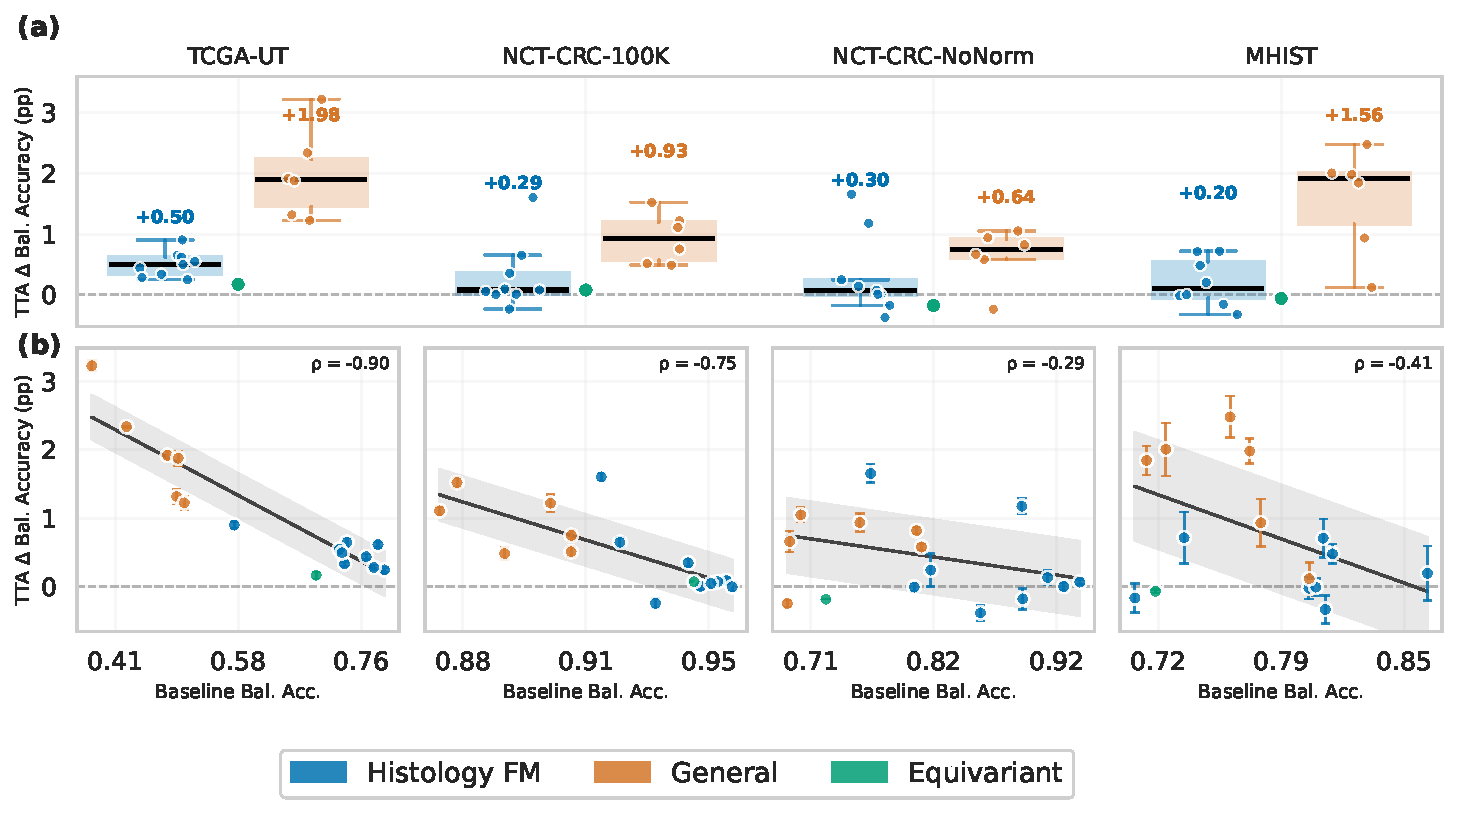
\includegraphics[width=1.0\linewidth]{latex/figures/figure2.pdf}
    \caption{$D_4$ test-time augmentation (TTA) consistently improves histopathology classifiers, with stronger gains for weaker baselines.
(a) Distribution of $\Delta_{\text{TTA}}$ in balanced accuracy (pp) across models for each dataset, split by model family (histology FMs vs. general-purpose backbones). Points show individual models; boxplots summarize the distribution; D4WRN (equivariant reference) exhibits near-zero gain by construction.
(b) Relationship between baseline balanced accuracy and $\Delta_{\text{TTA}}$ for each dataset: weaker baselines tend to benefit more from TTA. }
    \label{fig:tta_overview}
\end{figure*}

\begin{figure*}[!tb]
    \centering
    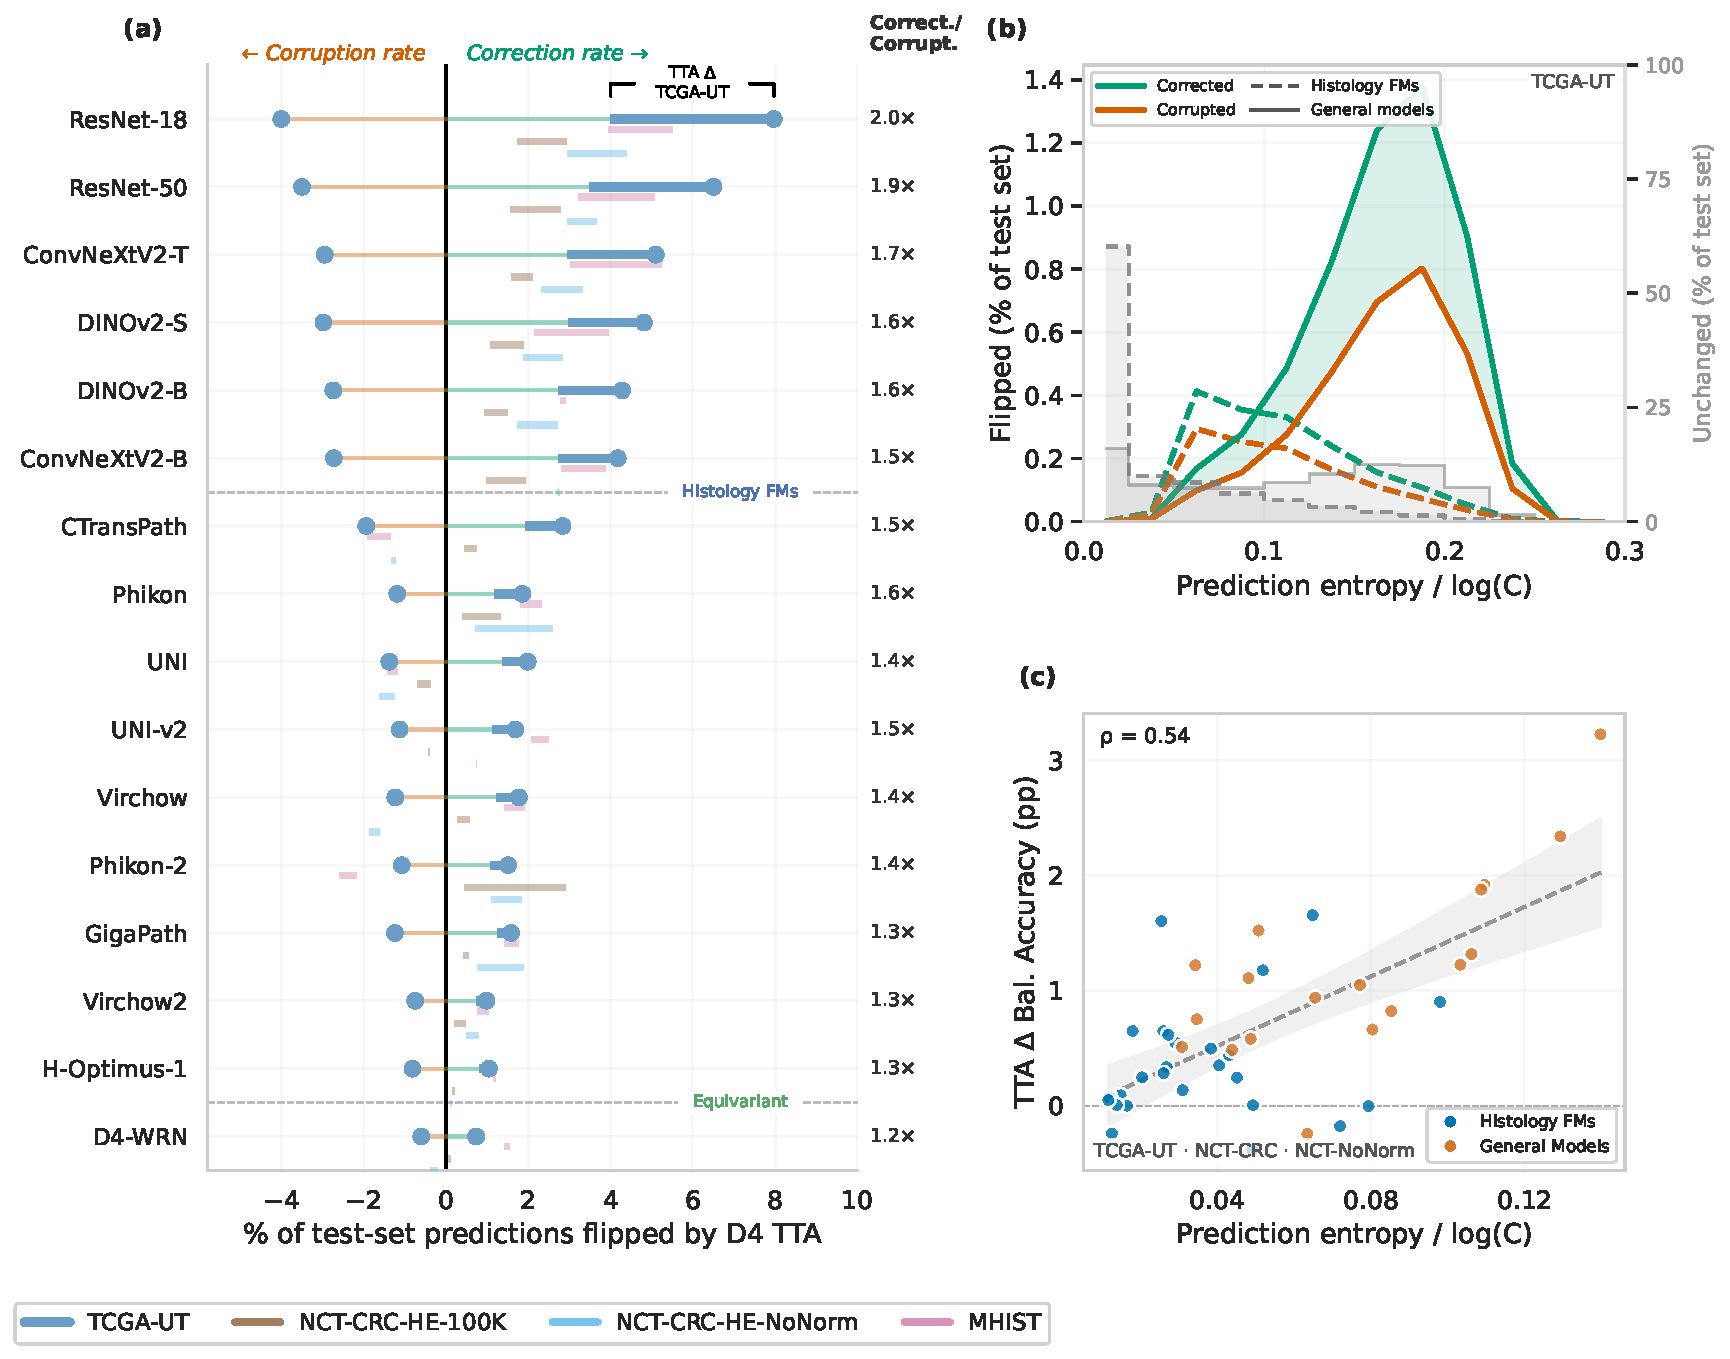
\includegraphics[width=1.0\linewidth]{latex/figures/figure3_journal.pdf}
    \caption{Prediction entropy explains $D_4$ TTA outcomes, where $\text{TTA}~\Delta$ denotes accuracy gain.
(a) For each model (TCGA-UT primary; other datasets shown as offset segments), we decompose the fraction of test predictions flipped by $D_4$ TTA into \emph{corrections} and \emph{corruptions}, sorting models by descending $\text{TTA}~\Delta$. The thick segment shows the net effect (correction $-$ corruption); the right margin reports the corrected/corrupted ratio. Models with small $\text{TTA}~\Delta$ exhibit low flip rates, consistent with increased $D_4$ prediction stability.
(b) Sample-level mechanism on TCGA-UT (31 classes). Binning samples by baseline softmax entropy (normalized by $\log C$) shows that both flips and net gains concentrate among high-entropy predictions: corrections and corruptions increase with entropy, but corrections increase more.
(c) Model-level predictability. Each point is one model $\times$ dataset combination (MHIST excluded). Mean prediction entropy strongly predicts $\text{TTA}~\Delta$ across models and datasets ($\rho = 0.54$), motivating entropy as a selection criterion for targeted TTA.}
    \label{fig:entropy}
\end{figure*}

% ============================================================================
\section{Methods}
\label{sec:methods}
% ============================================================================

\subsection{Models}

We evaluate 16 models spanning three categories (Table~\ref{tab:models}).

\textbf{Histology foundation models} (9 models) are used with frozen backbones and a trained linear classification head, following the standard linear probing protocol. This isolates the quality of the pretrained representations without confounding from downstream finetuning.

\textbf{General-purpose models} (6 models) pretrained on ImageNet are evaluated in both frozen (linear probe) and finetuned configurations to assess how downstream adaptation affects TTA benefit.

\textbf{Equivariant reference} (1 model): a $D_4$-equivariant Wide ResNet (D4WRN)~\citep{zagoruyko2016wide,weiler2019general} trained from scratch, providing an architecture with exact $D_4$-equivariance guarantees. We use it as an informative reference point for expected near-zero TTA benefit, noting that architectural and training-protocol differences limit direct comparison to pre-trained FMs (\ref{sec:d4wrn_caveats}).

\subsection{Datasets}
We evaluate on four tile-level classification datasets (Table~\ref{tab:datasets}) using the standard splits. TCGA-UT~\citep{komura2022universal} is split by patient (190{,}000/40{,}800/40{,}900 train/val/test tiles). For MHIST~\citep{wei2021petri}, we use the provided patient-disjoint split (2{,}175/977 train/test). For NCT-CRC-HE-100K and NCT-CRC-HE-NoNorm~\citep{kather2019predicting}, we use the standard split (100{,}000/7{,}180 train/test) with a fixed test set across runs. For all datasets, hyperparameters are selected by 3-fold cross-validation on the training set, and early stopping uses a held-out 10\% split carved from training data; the test split is never used during training. All reported metrics are computed on the held-out test split.

TCGA-UT is the most challenging benchmark with 31 fine-grained tissue classes across multiple organs. NCT-CRC-HE-100K and its non-normalized variant isolate the impact of stain normalization versus geometric TTA. MHIST is a binary task between Hyperplastic Polyp (HP) and Sessile Serrated Adenoma/Polyp (SSA).

\begin{table}[h] 
    \centering
    \caption{Datasets used for evaluation.}
    \label{tab:datasets}
    \vspace{6pt} 
    \small
    \begin{tabular}{@{}lrrr@{}} 
        \toprule
        Dataset & Classes & Test & Domain \\
        \midrule
        TCGA-UT           & 31 & 40.9k & Multi-organ \\
        NCT-CRC-HE-100K   & 9  & 7.2k  & Colorectal \\
        NCT-CRC-HE-NoNorm & 9  & 7.2k  & Colorectal \\
        MHIST             & 2  & 1k    & Colorectal polyp \\
        \bottomrule
    \end{tabular}
\end{table}

\subsection{TTA Strategies}

We evaluate three TTA strategies of increasing group size:

\begin{enumerate}
  \item None: standard single-view inference (baseline).
  \item \textbf{$V_4$} (4 views): horizontal flip, vertical flip, and both, forming the Klein four-group $V_4 \subset D_4$.
  \item \textbf{{$D_4$}} (8 views): all eight elements of the dihedral group, comprising four rotations (0\textdegree, 90\textdegree, 180\textdegree, 270\textdegree) composed with identity and horizontal flip.
\end{enumerate}

For each strategy, we evaluate four aggregation methods. Let $G$ denote the set of test-time views, with per-view logits $\ell_g\in\mathbb{R}^C$ and probabilities $p_g=\mathrm{softmax}(\ell_g)$. All sums below are over $g\in G$.
\begin{equation*}
\begin{aligned}
  a &= \mathrm{softmax}\!\left(\frac{1}{K}\sum_{g} \ell_g\right) && \text{(logit-mean)}\\
  a &= \frac{1}{K}\sum_{g} p_g && \text{(prob-mean)}\\
  a &= \frac{\sum_{g} w_g p_g}{\sum_{g} w_g},\qquad w_g = \max_{c}(p_g)_c && \text{(conf.-weighted)}\\
  \hat{y} &= \arg\max_{c}\, a_c && \text{(prediction)}
\end{aligned}
\end{equation*}
Majority vote predicts $\hat{y}=\operatorname*{mode}_{g}\bigl(\arg\max_{c}\,(p_g)_c\bigr)$.
Unless stated otherwise, we use logit-mean aggregation as the default; results for all aggregation variants are reported in Section~\ref{sec:results}.

Finally, we evaluate \textbf{selective TTA}, which adaptively applies full $D_4$ only to uncertain samples based on the entropy of the base-view prediction, trading off accuracy and inference cost (Section \ref{sec:selective}).


\subsection{Metrics}
We report \textbf{balanced accuracy} (macro-averaged recall) as our primary metric, since it weights all classes equally regardless of prevalence---critical for the imbalanced TCGA-UT dataset. For a $C$-class problem, balanced accuracy is
\begin{equation}
  \text{BalAcc}(f)=\frac{1}{C}\sum_{c=1}^{C}\frac{\text{TP}_c}{\text{TP}_c+\text{FN}_c}.
\end{equation}
The TTA benefit is quantified as the difference in balanced accuracy between TTA and baseline
\begin{equation}
  \Delta_{\text{TTA}} = \text{BalAcc}(f_{\text{TTA}}) - \text{BalAcc}(f_{\text{base}})
\end{equation}
reported in percentage points (pp). Positive values indicate TTA improvement.

For each TTA evaluation, we count \emph{corrections}: samples the baseline gets wrong but TTA gets right, and \emph{corruptions}: samples the baseline gets right but TTA gets wrong. The \textbf{correction ratio} $n_{\text{corrected}}/n_{\text{corrupted}} > 1$ indicates net benefit; it measures the \emph{quality} of TTA's prediction flips independently of their total count.

\textbf{Prediction entropy:} As an uncertainty proxy for selective TTA, we use the Shannon entropy of the single-view softmax $p(y\mid x)\in[0,1]^C$:
\begin{equation}
  H(x) = -\sum_{c=1}^{C} p(y=c\mid x)\,\log p(y=c\mid x),
\end{equation}
where $C$ is the number of classes and $\log$ is the natural logarithm. When comparing across datasets with different $C$, we report the normalized entropy $\tilde{H}(x)=H(x)/\log C\in[0,1]$.

\textbf{Orbit tightness (MPCS):} To quantify representation-level $D_4$ invariance (\S\ref{sec:orbit}), we ask how close a patch's eight $D_4$-view embeddings $z_g$ are to one another. Let $z_g$ be the frozen-backbone feature vector of view $g$. The mean pairwise cosine similarity (MPCS) averages, over all $\binom{8}{2}$ pairs of views, their cosine similarity,
\begin{equation}
  \text{MPCS} = \frac{1}{\binom{8}{2}} \sum_{g < g'} \frac{\langle z_g,\, z_{g'} \rangle}{\lVert z_g\rVert\,\lVert z_{g'}\rVert},
\end{equation}
which equals $1$ when all eight views point in the same direction (a perfectly invariant orbit).


\subsection{Training Protocol}

\textbf{Frozen backbones and trained heads.} We pre-extract patch embeddings once from each frozen backbone and train lightweight heads on top of the fixed features. Our primary head is a \emph{linear probe}: a single fully-connected layer trained by stochastic gradient descent (Adam) with cross-entropy loss---the standard self-supervised linear-probe protocol~\citep{oquab2023dinov2}. We additionally report one- and two-hidden-layer MLP probes and $k$-nearest-neighbour baselines ($k\in\{5,10\}$). For the linear and MLP heads, the learning rate ($\{10^{-3},\,3\times10^{-4}\}$) and weight decay ($\{10^{-4},\,10^{-3}\}$) are chosen by 3-fold cross-validation on the training set; the head is then trained on the full training set for up to 30 epochs with early stopping (patience 3) on a held-out 10\% validation split, using a fixed batch size of 512 across all models and datasets. Hyperparameters are selected once per (model, dataset, head) and shared across seeds.

\textbf{Finetuned general-purpose models.} The full network is optimized end-to-end with standard augmentation (random $D_4$ transforms; color jitter [brightness, contrast, saturation $\pm 0.25$; hue $\pm 0.05$]; random resized crops [scale $0.6$--$1.0$]; Gaussian blur), differential learning rates ($10^{-4}$ backbone, $10^{-3}$ head), cosine annealing over 20 epochs, batch size 64, early stopping patience 5, and label smoothing 0.1.

We run 5 random seeds ($\{0,1,2,3,42\}$) and report mean $\pm$ SEM; the $k$NN and all TTA evaluation are deterministic. Train/validation/test splits are fixed.

\subsection{Implementation}

All FMs are downloaded from HuggingFace. The $D_4$ equivariant model (D4WRN) was constructed using the escnn library \citep{weiler2019general} as a Wide ResNet-28-6 with steerable convolutions over the dihedral group $D_4$, yielding $12$M parameters, comparable to ResNet-18 - our weakest model. Feature maps use regular field types throughout, aggregating in the final stage to produce $D_4$-invariant embeddings. For the frozen-backbone experiments we pre-extract embeddings for all eight $D_4$ views of every test patch (and a single view of each training patch) in one batched, mixed-precision (FP16) pass per backbone, then train and evaluate all heads on the cached embeddings; per-strategy TTA results are obtained by aggregating the cached per-view embeddings/logits, avoiding redundant forward passes.

% ============================================================================
\section{Results}
\label{sec:results}
% ============================================================================
\subsection{TTA Consistently Improves Predictions}
Across the 15 frozen-backbone models and 4 datasets, $D_4$ TTA improves balanced accuracy in 50 of 60 model-dataset configurations, indicating that group-averaging is a reliable (if modest) post hoc gain (binomial test vs.\ 50\%: $p < 10^{-6}$). Improvements are larger for general-purpose backbones than for histology foundation models (Figure~\ref{fig:tta_overview}). We also observe a clear trend in $D_4$ \emph{prediction stability}: models with smaller $\Delta_{\text{TTA}}$ tend to show lower view-induced flip rates (Figure~\ref{fig:entropy}(a)), with D4WRN providing a near-zero reference point by construction.

Averaged across all four datasets and 5 seeds, histology FMs gain $+0.30$ pp (std $0.57$, $n=180$), $4.3\times$ smaller than general-purpose models ($+1.28$ pp; std $0.86$, $n=120$); the finetuned D4WRN reference gains $+0.17$ pp. The full per-model, per-dataset breakdown is reported in Table~\ref{tab:full_results}. Decomposing each $\Delta_{\text{TTA}}$ into the patches TTA \emph{corrects} versus \emph{corrupts} (Figure~\ref{fig:entropy}(a)), histology FMs show both fewer corrections and a lower net correction rate than general-purpose backbones, while D4WRN shows near-zero flips of either kind by construction (comparison not fully controlled; see \ref{sec:d4wrn_caveats}).

Breaking down by dataset, the same family gap holds:
\begin{itemize}
  \item \textbf{TCGA-UT} (31 classes): histology FMs $+0.50$ pp vs.\ general $+1.98$ pp.
  \item \textbf{NCT-CRC-HE-100K} (9 classes, normalized): histology FMs $+0.29$ pp vs.\ general $+0.93$ pp.
  \item \textbf{NCT-CRC-HE-NoNorm} (9 classes, raw): histology FMs $+0.30$ pp vs.\ general $+0.64$ pp.
  \item \textbf{MHIST} (binary): histology FMs $+0.11$ pp vs.\ general $+1.56$ pp.
\end{itemize}
The family gap is significant by a rank-based test that makes no linearity assumption (general $>$ FM, Mann--Whitney U/Wilcoxon rank-sum test $p < 10^{-3}$ on TCGA-UT), and the association between $\Delta_{\text{TTA}}$ and baseline accuracy is negative in all four datasets (Spearman rank correlation $\rho$ from $-0.4$ to $-0.9$; Fisher's method for combining $p$-values gives $p < 10^{-7}$). These conclusions are robust to the choice of lightweight classifier head on top of frozen features (linear vs.\ MLP vs.\ $k$NN), with head-family averages summarized in Table~\ref{tab:head_comparison}.

We test whether the decline in TTA benefit for stronger models is simply due to reduced error (less ``headroom'') by measuring the net correction rate per dataset. On TCGA-UT, the corrected-to-corrupted ratio becomes less favorable as model quality increases (roughly from $\approx\!2{:}1$ for the weakest backbones to $\approx\!1.3{:}1$ for the strongest FMs), suggesting that the remaining mistakes of stronger models are less often fixable by simple geometric averaging. Consistent with this, the exactly $D_4$-equivariant D4WRN shows near-zero TTA benefit, pointing to learned invariance (rather than accuracy alone) as a key factor.

To clarify where the remaining gains occur, we next show that TTA benefit concentrates among high-entropy (uncertain) predictions (Figure~\ref{fig:entropy}(b--c)). Table~\ref{tab:full_results} reports the per-model results on TCGA-UT: general-purpose backbones tend to benefit the most, whereas histology foundation models---especially the largest ones---show consistently smaller improvements. Within the histology models, the ranking broadly tracks model scale and pretraining volume (e.g., CTransPath and smaller FMs benefit more than the largest, most heavily pretrained transformers).


\begin{figure*}[!tb]
    \centering
    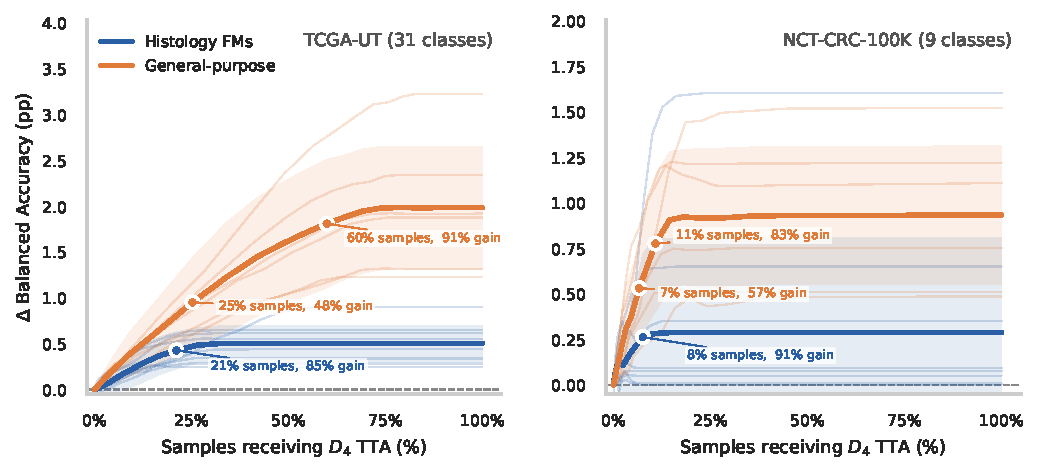
\includegraphics[width=1.0\linewidth]{latex/figures/figure4_selective_pareto.pdf}
    \caption{Selective TTA accuracy--efficiency trade-off on TCGA-UT. Each point corresponds to an entropy threshold $t$ for routing samples to full $D_4$ TTA; lower $t$ applies TTA to more samples (higher cost) and vice versa. Histology FMs recover nearly the full $D_4$ benefit while saving a substantial fraction of forward passes.}
    \label{fig:selective_pareto}
\end{figure*}

\paragraph{D4WRN as a near-zero reference.}
\label{sec:d4wrn_caveats}

The D4WRN, exactly $D_4$-equivariant by construction, shows a near-zero mean TTA benefit of $+0.17$ pp (TCGA-UT: $+0.17$ pp, NCT-CRC-HE-100K: $+0.08$ pp, NCT-CRC-HE-NoNorm: $-0.18$ pp), despite being much smaller (${\sim}12$M parameters) and no large-scale pretraining. We treat it as an informative but uncontrolled reference, since it differs from histology FMs in architecture (Wide ResNet vs.\ ViT), scale (86M--1.1B parameters), and training protocol. Our primary evidence for learned invariance in histology FMs instead comes from the convergence of small TTA deltas, high view agreement, and a $4.3\times$ gain gap relative to general-purpose models.

\subsection{Frozen Backbones Benefit More Than Finetuned}
\label{sec:frozen_ft}

We evaluate the six general-purpose backbones in both frozen (linear-probe) and finetuned (end-to-end) configurations. The finetuning runs cover TCGA-UT, NCT-CRC-HE-100K, and NCT-CRC-HE-NoNorm (MHIST excluded), so for a like-for-like comparison we restrict both configurations to these three datasets. On this matched set, frozen backbones gain $+1.19$ pp from $D_4$ TTA versus $+0.56$ pp when finetuned---a $2.1\times$ reduction. Finetuning simultaneously raises the mean baseline balanced accuracy from $69.9\%$ to $78.7\%$ ($+8.8$ pp), so the shrinking TTA benefit accompanies a stronger base model. This is consistent with the hypothesis that finetuning on augmented histopathology data teaches the network additional rotational invariance, partially absorbing the benefit that $D_4$ TTA would otherwise provide---the same mechanism we attribute to large-scale self-supervised pretraining in the histology FMs (\S\ref{sec:discussion}).


\subsection{Strategy Progression: Diminishing Returns Beyond Flips}

Increasing TTA group size from the Klein four-group $V_4$ (4 views: identity, both flips, and 180\textdegree rotation) to the full dihedral group $D_4$ (8 views) yields diminishing returns. Across the 15 frozen linear probes and 4 datasets, $V_4$ averages $+0.53$ pp versus $+0.69$ pp for $D_4$---an additional $+0.16$ pp for doubling the number of forward passes. The increment is concentrated in general-purpose backbones ($V_4$ $+0.94$ vs.\ $D_4$ $+1.28$ pp), whereas histology FMs gain almost everything from flips alone ($V_4$ $+0.26$ vs.\ $D_4$ $+0.30$ pp): the 90\textdegree and 270\textdegree rotations add only ${\sim}0.05$ pp. This is consistent with self-supervised pretraining with rotation augmentation having already captured the proper-rotation symmetries, leaving little for $D_4$ to recover beyond reflections. Per-model $V_4$ and $D_4$ deltas are reported in Table~\ref{tab:full_results}.
Among $D_4$ aggregation methods, logit-mean, probability-mean, and confidence-weighted averaging perform comparably (within $\sim 0.03$ pp), while hard voting is slightly worse; we use logit-mean throughout unless stated otherwise.



\subsection{TTA Corrects More Than It Corrupts}

TTA with $D_4$ produces an overall net correction ratio (corrected/corrupted) of 1.60 (see Figure~\ref{fig:entropy}(a)), and exceeds 1 for both model families (general-purpose: 1.69, histology FMs: 1.44). TTA is thus a ``safe'' technique that reliably corrects more than it corrupts, even when overall gains are small.


\subsection{Agreement Rate Quantifies Prediction-Level Invariance}
\label{sec:agreement}

Histology FMs achieve a mean base-vs-$D_4$ prediction agreement rate of 97.0\% (range 91.8\%--99.7\%) compared to 91.2\% (range 74.3\%--97.5\%) for general-purpose models. This gap quantifies $D_4$ stability at the \emph{prediction} level---which, as \S\ref{sec:orbit} shows, is a property of the classifier's decision geometry and is \emph{not} explained by embedding-space (representation) invariance---independent of the D4WRN comparison caveats in \S\ref{sec:d4wrn_caveats}. Within the FM family the ranking tracks model scale: CTransPath shows the lowest agreement (91.8\% on TCGA-UT) while the largest models (Virchow-v2, H-Optimus-1) exceed 98\%.

Baseline softmax entropy also predicts prediction \emph{correctness}, not just TTA flip events. Across model $\times$ dataset combinations, entropy achieves an AUROC of $0.849 \pm 0.058$ for discriminating incorrect from correct predictions in histology FMs (general-purpose: $0.816 \pm 0.049$). Incorrect predictions carry $4.3\times$ higher normalized entropy than correct ones for FMs ($2.6\times$ for general-purpose models), suggesting FM softmax is better calibrated: when the model is uncertain, it is substantially more likely to be wrong. This sample-level relationship motivates the entropy routing in \S\ref{sec:selective}; Figure~\ref{fig:entropy}(b--c) shows how this uncertainty concentrates TTA benefit.


\subsection{Selective TTA Preserves Benefits at Reduced Inference Cost}
\label{sec:selective}

Histology FM predictions are highly confident (low entropy) on the large majority of patches, so full $D_4$ TTA adds redundant computation for most inputs. We exploit this by applying selective TTA: single-view inference for samples whose base-view softmax entropy falls below a threshold, and full $D_4$ for uncertain samples:
\begin{equation}
  \hat{f}_{\text{sel}}(x) =
  \begin{dcases}
    f(x) & \text{if } H[\sigma(f(x))] \le t \cdot \ln C \\
    \frac{1}{|G|} \sum_{g \in G} f(g \cdot x) & \text{otherwise}
  \end{dcases}
  \label{eq:selective}
\end{equation}
where normalizing by $\ln C$ makes the threshold $t \in [0,1]$ comparable across datasets with different numbers of classes $C$. Figure~\ref{fig:selective_pareto} shows the efficiency--accuracy tradeoff curve (Pareto frontier) for selected histology FMs and general-purpose models on TCGA-UT.

For \textbf{histology FMs} (frozen backbone, averaged across Phikon-v2, GigaPath, and H-Optimus-1; full-$D_4$ benefit $+0.34$ pp):
\begin{itemize}
  \item At $t = 0.3$: only 13\% of samples receive TTA (saving 87\% of forward passes), recovering $+0.24$ pp---about 69\% of the full benefit.
  \item At $t = 0.5$: 3\% of samples receive TTA (97\% of passes saved), recovering $+0.031$ pp.
\end{itemize}
Because these FMs produce low-entropy predictions on most patches, the recoverable TTA benefit is concentrated in the small subset of high-entropy patches; selective TTA therefore captures most of the full-$D_4$ gain at a fraction of the inference cost.

For general-purpose models, savings are more modest as their higher disagreement means more samples genuinely benefit: at $t = 0.3$, 65\% of samples receive TTA and recover 95\% of the benefit. Base-view entropy is thus an effective routing signal, concentrating TTA cost on the few unstable predictions. Entropy works here because it is a proxy for proximity to a decision boundary---the geometric quantity that actually determines whether $D_4$ averaging flips a prediction (\S\ref{sec:orbit})---so the base-view margin to the nearest boundary is an equivalent, equal-cost routing signal. Routing can concentrate the flips but not improve their quality: among patches that flip, no base-view signal (entropy or margin) separates beneficial corrections from harmful corruptions (AUROC $\approx 0.50$), so the net benefit of selective TTA is bounded by the intrinsic correction-to-corruption ratio of the flipped set. A natural hypothesis is that representation-level $D_4$ invariance should predict which models benefit; we test this next.


\subsection{A Flip Occurs When the Orbit Straddles the Decision Boundary}
\label{sec:orbit}

We first test the natural hypothesis that representation-level $D_4$ invariance explains TTA benefit, measuring orbit tightness by MPCS (\S\ref{sec:methods}). It does not: histology FMs are \emph{not} more orbit-invariant than general-purpose models (mean MPCS $0.946$ vs.\ $0.950$), and per patch, orbit tightness barely separates flipped from unflipped predictions (AUROC $0.57$, near chance). The architecturally $D_4$-equivariant D4WRN is the one exception, collapsing each orbit almost to a point (MPCS $\approx 0.999$). This confirms that MPCS detects invariance when it is present, and that FMs' high prediction agreement (\S\ref{sec:agreement}) is \emph{not} embedding-level invariance.

A flip happens only when the orbit straddles the decision boundary between the base-view top-two classes. How far the base-view embedding sits from that boundary (the geometric margin) predicts flips at AUROC $0.949$ per patch, matching softmax entropy ($0.919$) but computed directly from the classifier geometry; scaling that margin by the orbit's spread along the boundary normal (the \emph{straddle ratio}) raises this to $0.955$.

This recasts the FM/general gap as a margin effect, not an invariance one. Since orbit size is essentially equal across families, FMs flip less only because their more separable representations place the same-sized orbit farther from decision boundaries, crossing one $3.4\times$ less often than general models on TCGA-UT ($9.9\%$ vs.\ $33.7\%$ of patches). Prediction stability under $D_4$ is therefore a property of where the orbit sits relative to the boundary, set jointly by classification margin and orbit geometry, rather than by backbone invariance alone.

\subsection{Stain Normalization Matters More Than Geometric TTA}

Comparing NCT-CRC-HE-100K (stain-normalized) with NCT-CRC-HE-NoNorm reveals that stain normalization has a far larger effect than geometric TTA. For histology FMs, the mean baseline balanced accuracy drops by $7.2$ pp without stain normalization (94.0\% $\to$ 86.9\%), while TTA recovers only $+0.30$ pp on the non-normalized data (compared to $+0.29$ pp on normalized data).

This ${\approx}24\times$ ratio (7.2 pp stain effect vs.\ 0.30 pp TTA effect) suggests that, on these benchmarks, geometric $D_4$ invariance is not the dominant source of error for modern histology FMs, whereas stain and scanner robustness remains a significant open challenge.

While the preceding results treat tiles as independent samples, clinical deployment and many research pipelines operate on whole-slide images. We therefore ask whether the (modest) tile-level corrections induced by $D_4$ averaging translate into improvements for slide-level prediction.

% ============================================================================

\section{WSI-Level Analysis: From Tiles to Slides}
\label{sec:wsi}

\subsection{Datasets and Setup}

\textbf{Camelyon17}~\citep{bandi2018camelyon17} provides 500 H\&E-stained lymph-node WSIs from 5 acquisition centers (100 slides, 20 patients per center); 50 slides carry pixel-level lesion polygon annotations.
The frozen UNI patch probe (binary tumor/normal) is evaluated leave-one-patient-out over the 50 annotated slides to avoid leakage. For slide-level MIL we use the standard domain-generalization split---train on centers 0--3, test on the unseen-scanner center 4 (100 slides).

\textbf{PANDA}~\citep{bulten2022artificial} provides prostate biopsy WSIs with pixel-level Gleason-grade annotations.
We binarise annotations into cancer / non-cancer and extract $512\times512$ patches at $20\times$ magnification, yielding 10,353 slides with at least one patch ($3{,}721$ with $\geq1$ cancer patch).


\subsection{Patch Corrections Do Not Transfer to Slide-Level MIL}

We ask whether the tile-level corrections induced by $D_4$ TTA carry over to slide-level prediction. Adding $D_4$ TTA to a trained ABMIL~\citep{ilse2018abmil} does not change bag-level performance beyond run-to-run variance. On Camelyon17 this null holds across six backbones spanning weak general-purpose models to strong FMs (ResNet-50, ConvNeXtV2, Phikon-v2, GigaPath, UNI, Virchow-v2): every test-AUC change is at most $0.009$ (range $-0.005$ to $+0.009$, e.g.\ UNI $0.972 \to 0.974$), in each case smaller than the seed-to-seed standard deviation. On PANDA, ABMIL quadratic-weighted $\kappa$ is $0.901$ with TTA versus $0.905$ without (UNI, 3 folds).

The null is structural rather than a property of any one backbone: it holds even for ResNet-50 and ConvNeXtV2, whose patch features are far from $D_4$-invariant and which gain the most from patch-level TTA (\S\ref{sec:results}). ABMIL pools hundreds to thousands of patches per slide, and this aggregation already averages out the small, largely cancelling per-patch perturbations that $D_4$ introduces, leaving the bag representation essentially unchanged. The effect is \emph{not} that attention ignores the affected patches: using the patch probe as a diagnostic, the ${\approx}0.1\%$ of patches whose prediction $D_4$ would flip fall in the top decile of UNI ABMIL attention. They are simply too few to move the pooled logit.

At the patch level, the corrections are modest and headroom-gated, as on the tile benchmarks. Leave-one-patient-out per-slide Dice improves on 59\% of PANDA cancer slides (mean $+0.66$\,pp; $n=3{,}721$), with the gain concentrated on poorly-segmented slides ($+1.0$\,pp in the lowest baseline-Dice tertile versus $+0.25$\,pp in the highest). The frozen UNI probe already segments tumor well, leaving little headroom for $D_4$ averaging to recover.



% ============================================================================

\section{Discussion}
\label{sec:discussion}
% ============================================================================

\subsection{Prediction Stability Reflects Joint Backbone--Classifier Geometry}

Our central finding is that histology foundation models exhibit near-\emph{invariant} \emph{predictions} under $D_4$ transforms (97.0\% base-vs-$D_4$ agreement; \S\ref{sec:agreement}), so the incremental accuracy gains from $D_4$ ensembling are typically small. This rests on converging evidence: small TTA deltas, high view agreement, and correction-dominated error profiles.

A $D_4$ orbit flips a prediction only when it \emph{straddles} a decision boundary, which depends on the orbit's spread \emph{and} its margin jointly (the straddle ratio, margin divided by orbit spread along the boundary normal), not on either alone---a property of the joint backbone--classifier geometry rather than of the backbone in isolation. This admits two routes to stability. The architecturally $D_4$-equivariant D4WRN takes the \emph{invariance} route: its orbits collapse to a point (MPCS $\approx 0.999$; \S\ref{sec:orbit}), so views cannot cross a boundary regardless of margin. Histology FMs take the \emph{margin} route: their embeddings move under $D_4$ as much as general-purpose models' (orbit tightness is decoupled from TTA benefit), but their more separable, larger-margin representations keep the same-sized orbit on one side of the boundary. A plausible source of these margins is the pretraining regime---heavy $D_4$ augmentation on orientation-diverse slides, expected to promote $D_4$-stable behavior~\citep{lyle2020benefits}---but the resulting stability is a downstream property of classification margin, not of representation-level invariance in the backbone.

\subsection{When Does TTA Still Help?}

Despite the overall small effect, TTA remains valuable in specific scenarios:

\begin{enumerate}
  \item \textbf{General-purpose backbones}: When histology-specific FMs are unavailable or a general ViT/ConvNeXt/ResNet is used, TTA provides meaningful gains ($+1.28$ pp).
  \item \textbf{Frozen linear probes}: On the datasets where both configurations were run, linear probes on frozen features benefit more than finetuned models ($+1.19$ vs.\ $+0.56$ pp), suggesting TTA partially compensates for the classifier's inability to learn invariance from limited data.
  \item \textbf{High-stakes applications}: When $+0.3$ pp matters---e.g., screening programs processing millions of tiles---the deterministic, risk-free nature of TTA (correction ratio consistently $> 1$) may justify the $8\times$ computational overhead.
\end{enumerate}

\subsection{Practical Recommendations}

For histology FM workflows, the $+0.30$ pp average gain rarely justifies $8\times$ inference cost; skip TTA by default. If TTA is used, use probability-mean aggregation. Stain normalization (\S\ref{sec:results}) is a higher-impact priority for these models.

When TTA is used, apply it selectively (\ref{sec:selective}): route samples to full $D_4$ only if their single-view normalized entropy exceeds a threshold $t$. Because histology FM predictions are highly confident, very few patches need TTA: at $t = 0.3$ only ${\sim}13\%$ of patches are augmented (87\% of forward passes saved) while recovering ${\sim}70\%$ of the full benefit. For general-purpose models the operating point shifts---$t = 0.3$ augments $65\%$ of patches and recovers $95\%$ of the benefit---but the principle holds across model families. In practice, $t = 0.3$--$0.5$ is a robust default; users can tune on a held-out validation set if a tighter efficiency target is required.

\subsection{Limitations}

Our study has several limitations. First, training protocol is a confound when comparing histology FMs (frozen linear probes only) to general-purpose models (frozen and finetuned): on the matched datasets, finetuning reduces mean TTA gain from $+1.19$ pp to $+0.56$ pp, so part of the FM vs.\ general-purpose gap may reflect downstream adaptation rather than pretraining-acquired invariance alone. Second, the D4WRN comparison is uncontrolled (architecture, scale, and training protocol all differ; \S\ref{sec:d4wrn_caveats}); a matched equivariant control is left to future work. Third, our WSI analysis (\S\ref{sec:wsi}) is limited to two datasets with patch-level annotations (Camelyon17, PANDA); generalization to other cancer types and scanners remains to be evaluated. Fourth, our statistical tests are uncorrected paired $t$-tests; future work could apply multiple-comparison corrections. Fifth, datasets are limited to H\&E staining; IHC or special stains may have different symmetry properties.


\subsection{Future Directions}

Our results point to several promising research directions:

\begin{itemize}
  \item \textbf{Stain-equivariant architectures}: Analogous to $D_4$-equivariant networks for geometric transforms, architectures with built-in stain invariance could address the larger remaining gap.
  \item \textbf{Adaptive thresholding for selective TTA}: We demonstrate entropy-based routing at fixed thresholds (\ref{sec:selective}); future work could learn per-dataset or per-class thresholds, or jointly optimize the routing policy with the classifier head.
  \item \textbf{Matched equivariant controls}: A $D_4$-equivariant ViT variant evaluated via frozen linear probe would provide a controlled floor for TTA benefit, isolating the effect of architectural equivariance from training protocol confounds.
  \item \textbf{Invariance probing}: Developing systematic benchmarks for measuring the degree of learned invariance across different transformation groups (geometric, photometric, stain) would help characterize FM capabilities beyond standard accuracy metrics.
\end{itemize}

% ============================================================================
\section{Conclusion}
\label{sec:conclusion}
% ============================================================================

We have presented the first large-scale evaluation of test-time augmentation across 16 vision models and 4 histopathology datasets. Our results show that modern histology foundation models exhibit high prediction stability under $D_4$ transforms and gain only $+0.30$ pp from $D_4$ TTA---a $4.3\times$ smaller benefit than general-purpose models. While TTA remains a safe and reliable technique---improving 83\% of configurations and correcting more predictions than it corrupts---its marginal benefit for histology FMs suggests that geometric $D_4$ robustness is often not the primary performance bottleneck for tile-level classification with modern FMs.

We further show that entropy-based selective TTA---routing only uncertain samples to full $D_4$---recovers most of the TTA benefit for histology FMs while augmenting only ${\sim}13\%$ of patches ($t=0.3$; 87\% of forward passes saved), providing a practical path to reduced-cost TTA when inference budget is constrained. By contrast, stain normalization has a far larger effect on these models, pointing to stain and scanner robustness as the more pressing open challenge. We release our complete evaluation framework to facilitate further research into invariance properties of histopathology foundation models.



%%%%%%%%%%%%%%%%%%%%%%%%%%%%%%%%%%%%%%%%%%%%%%%%%%%%%%%%%%%%%%%%%%%%%%%
% Mandatory Sections. Please complete, especially for final publication
%%%%%%%%%%%%%%%%%%%%%%%%%%%%%%%%%%%%%%%%%%%%%%%%%%%%%%%%%%%%%%%%%%%%%%%

% Acknowledgements.
% Please include any funding, intellectual contributions not included in the authorship, and any other acknowledgements.
\acks{We utilized generative artificial intelligence (AI) to assist in creating and refining code segments based on specified tasks, including debugging, editing, and autocompleting code. Additionally, generative AI tools were used to help
structure sentences and perform grammar checks. The conceptualization and ideation, as well as all instructions given to the AI, were exclusively the result of the authors’
creative and intellectual input. We take full responsibility for reviewing and ensuring the accuracy and quality of all AI-generated content included in this work}

% Ethical Standards.
% Please edit with the appropriate ethics considerations for your work. Include any pertinent IRB information, etc.
%
% Please note that the submission requirements included:
% The work presented must follow appropriate ethical standards in conducting research and writing the manuscript, following all applicable laws and regulations regarding treatment of animals or human subjects.
\ethics{The work follows appropriate ethical standards in conducting research and writing the manuscript, following all applicable laws and regulations regarding treatment of animals or human subjects.}

% Conflict of Interest
% Declaration of possible conflicts of interest: Authors must disclose any financial, organisational, commercial or personal conflicts of interest that might bias their work.
% If no conflicts, please say "We declare we don't have conflicts of interest."
\coi{We declare we don't have conflicts of interest.}

% Data availability
\data{This paper utilizes data and models that are available on Huggingface and GitHub.}

\bibliography{sample}

% Manual newpage inserted to improve layout of sample file - not
% needed in general before appendices.
% \newpage

% Appendix is optional
\clearpage
\appendix
\onecolumn

\section{Additional Tables}\suppressfloats[t]
% Auto-generated by utils/generate_tables.py — do not edit by hand.
\begin{table*}[t]
\centering
\caption{Per-model TTA results across all four datasets (frozen backbone / SGD linear probe,
mean-probability aggregation, 5 seeds). \textit{Base}: no-TTA balanced accuracy (\%).
$V_4$ and $D_4$: change in percentage points from 4-view (flips) and 8-view (full dihedral)
TTA respectively. Significance of $D_4\,\Delta$ vs.\ zero (two-sided paired $t$-test, $n=5$ seeds,
uncorrected): $^{*}p<0.05$, $^{**}p<0.01$, $^{***}p<0.001$.
Best $D_4$ $\Delta$ per dataset in \textbf{bold}. Class counts: TCGA-UT 31, NCT-100K / NCT-NoNorm 9, MHIST 2.
D4WRN is finetuned (seeds vary by dataset; see $^\dagger$) and shown as an
uncontrolled equivariant reference (see \S\ref{sec:d4wrn_caveats}).}
\label{tab:full_results}
\vspace{4pt}
\small
\setlength{\tabcolsep}{4pt}
\begin{tabular}{@{}llcccccccccccc@{}}
\toprule
& & \multicolumn{3}{c}{TCGA-UT} & \multicolumn{3}{c}{NCT-100K} & \multicolumn{3}{c}{NCT-NoNorm} & \multicolumn{3}{c}{MHIST} \\
\cmidrule(lr){3-5} \cmidrule(lr){6-8} \cmidrule(lr){9-11} \cmidrule(lr){12-14}
Type & Model & Base & $V_4$ & $D_4$ & Base & $V_4$ & $D_4$ & Base & $V_4$ & $D_4$ & Base & $V_4$ & $D_4$ \\
\midrule
\multicolumn{14}{@{}l}{\textit{General-purpose}} \\
& ResNet-18          & 37.5 & $+2.48$ & \textbf{$+3.23^{***}$} & 86.9 & $+1.06$ & $+1.11^{***}$ & 69.5 & $+0.72$ & $+0.66^{*}$ & 71.8 & $+0.94$ & $+1.84^{***}$ \\
& ResNet-50          & 42.5 & $+1.92$ & $+2.34^{***}$ & 87.4 & $+1.10$ & $+1.52^{***}$ & 80.4 & $+0.85$ & $+0.82^{***}$ & 72.8 & $+1.27$ & $+2.01^{**}$ \\
& ConvNeXtV2-Tiny    & 48.3 & $+1.31$ & $+1.92^{***}$ & 88.8 & $+0.43$ & $+0.49^{**}$ & 70.4 & $+0.47$ & $+1.05^{***}$ & 76.2 & $+1.43$ & \textbf{$+2.48^{**}$} \\
& ConvNeXtV2-Base    & 49.6 & $+1.01$ & $+1.32^{***}$ & 90.1 & $+0.83$ & $+1.22^{***}$ & 69.3 & $+0.20$ & $-0.24^{**}$ & 77.8 & $+0.43$ & $+0.94$ \\
& DINOv2-S           & 49.8 & $+1.27$ & $+1.88^{***}$ & 90.7 & $+0.78$ & $+0.75^{***}$ & 75.5 & $+0.40$ & $+0.94^{**}$ & 77.3 & $+1.28$ & $+1.98^{***}$ \\
& DINOv2-B           & 50.7 & $+0.90$ & $+1.23^{***}$ & 90.7 & $+0.68$ & $+0.51^{**}$ & 80.8 & $+0.64$ & $+0.58^{***}$ & 80.4 & $+0.11$ & $+0.12$ \\
\addlinespace[3pt]
\multicolumn{14}{@{}l}{\textit{Histology foundation models}} \\
& CTransPath         & 57.9 & $+0.67$ & $+0.90^{***}$ & 94.2 & $+0.48$ & $+0.35^{**}$ & 80.2 & $+0.27$ & $+0.00$ & 59.0 & $+0.09$ & $-0.58$ \\
& Phikon             & 74.0 & $+0.45$ & $+0.65^{***}$ & 92.2 & $+0.48$ & $+0.65^{***}$ & 76.4 & $+2.34$ & \textbf{$+1.66^{***}$} & 73.8 & $+0.28$ & $+0.72$ \\
& Phikon-v2          & 76.8 & $+0.31$ & $+0.44^{***}$ & 91.6 & $+0.89$ & \textbf{$+1.60^{***}$} & 89.5 & $-0.14$ & $-0.17$ & 71.2 & $-0.05$ & $-0.16$ \\
& UNI                & 72.9 & $+0.41$ & $+0.55^{***}$ & 93.2 & $-0.26$ & $-0.24^{*}$ & 85.8 & $-0.35$ & $-0.38^{*}$ & 81.2 & $-0.50$ & $-0.33$ \\
& UNI-v2             & 78.5 & $+0.51$ & $+0.62^{***}$ & 95.5 & $-0.04$ & $+0.00$ & 93.0 & $+0.13$ & $+0.01$ & 81.1 & $+0.97$ & $+0.71$ \\
& Virchow            & 73.3 & $+0.46$ & $+0.50^{***}$ & 94.5 & $+0.01$ & $+0.01$ & 81.6 & $-0.17$ & $+0.25$ & 81.6 & $+0.42$ & $+0.48^{*}$ \\
& Virchow-v2         & 77.9 & $+0.20$ & $+0.28^{***}$ & 94.8 & $+0.13$ & $+0.05$ & 91.6 & $+0.14$ & $+0.14$ & 86.7 & $+0.35$ & $+0.20$ \\
& GigaPath           & 73.7 & $+0.24$ & $+0.34^{***}$ & 95.3 & $+0.05$ & $+0.09$ & 89.4 & $+0.38$ & $+1.18^{***}$ & 80.4 & $-0.37$ & $-0.02$ \\
& H-Optimus-1        & 79.4 & $+0.13$ & $+0.25^{**}$ & 95.0 & $+0.12$ & $+0.08$ & 94.4 & $+0.13$ & $+0.07$ & 80.8 & $+0.05$ & $+0.00$ \\
\addlinespace[3pt]
\multicolumn{14}{@{}l}{\textit{Equivariant reference}} \\
& D4WRN$^\dagger$    & 69.6 & $+0.17$ & $+0.17$ & 94.3 & $+0.08$ & $+0.08$ & 72.6 & $-0.19$ & $-0.18$ & 72.3 & $-0.10$ & $-0.06$ \\
\bottomrule
\end{tabular}
\vspace{4pt}

\noindent\small$^\dagger$ D4WRN is evaluated in finetuned mode; number of seeds varies by dataset
(TCGA-UT: 5, NCT-CRC-100K/MHIST: 2, NCT-CRC-NoNorm: 1). All other models use frozen backbone
with SGD linear probe (5 seeds).
\end{table*}


% Auto-generated by utils/generate_tables.py — do not edit by hand.
\begin{table*}[t]
\centering
\caption{Mean $D_4$ TTA benefit ($\Delta$ balanced accuracy, pp) by classifier head type and
model family (frozen backbone, mean-probability aggregation). Values averaged over all models
within each family and 5 seeds (kNN: 1 seed, deterministic).
\textit{Base}: mean no-TTA balanced accuracy (\%). $\Delta$: pp gain from $D_4$ TTA.}
\label{tab:head_comparison}
\vspace{4pt}
\small
\setlength{\tabcolsep}{4pt}
\begin{tabular}{@{}llcccccccc@{}}
\toprule
& & \multicolumn{2}{c}{TCGA-UT (31 cls)} & \multicolumn{2}{c}{NCT-CRC-100K (9 cls)} & \multicolumn{2}{c}{NCT-CRC-NoNorm (9 cls)} & \multicolumn{2}{c}{MHIST (2 cls)} \\
\cmidrule(lr){3-4} \cmidrule(lr){5-6} \cmidrule(lr){7-8} \cmidrule(lr){9-10}
Family & Head & Base & $\Delta$ & Base & $\Delta$ & Base & $\Delta$ & Base & $\Delta$ \\
\midrule
\multicolumn{10}{@{}l}{\textit{General-purpose models}} \\
& kNN ($k$=10)       & 27.6 & $+0.86$ & 83.9 & $+0.99$ & 80.3 & $+1.19$ & 71.9 & $+0.95$ \\
& Linear             & 46.4 & $+1.98$ & 89.1 & $+0.93$ & 74.3 & $+0.64$ & 76.1 & $+1.56$ \\
& MLP-1h             & 48.4 & $+2.33$ & 89.8 & $+1.17$ & 73.8 & $+1.06$ & 76.8 & $+1.73$ \\
& MLP-2h             & 48.3 & $+2.38$ & 89.6 & $+1.13$ & 73.5 & $+1.37$ & 77.3 & $+1.67$ \\
\addlinespace[3pt]
\multicolumn{10}{@{}l}{\textit{Histology FMs}} \\
& kNN ($k$=10)       & 63.0 & $+0.32$ & 94.2 & $+0.23$ & 89.9 & $-0.01$ & 73.8 & $-0.14$ \\
& Linear             & 73.8 & $+0.50$ & 94.0 & $+0.29$ & 86.9 & $+0.30$ & 77.3 & $+0.11$ \\
& MLP-1h             & 74.5 & $+0.39$ & 94.0 & $+0.30$ & 86.4 & $+0.39$ & 80.2 & $+0.33$ \\
& MLP-2h             & 74.5 & $+0.40$ & 93.9 & $+0.36$ & 85.5 & $+0.48$ & 80.0 & $+0.45$ \\
\bottomrule
\end{tabular}
\end{table*}


\end{document}
